% !TEX TS-program = xelatex
% !TEX encoding = UTF-8

\documentclass{ctexart}
\usepackage{note}

\title{Multi-Task Learning笔记}
\author{Fw[a]rd\thanks{这篇文章的内容以GPLv2协议释出}}
\date{2021年6月9日}

\begin{document}
\maketitle

\section{因缘}
因为某个项目的原因,需要考虑多个loss的平衡问题。在\href{https://www.zhihu.com/question/375794498}{知乎}用户的推荐下阅读了:

\begin{itemize}
    \item Multi-Task Learning Using Uncertainty to Weigh Losses for Scene Geometry and Semantics\cite{Kendall18Uncertainty}
    \item GradNorm: Gradient Normalization for Adaptive Loss Balancing in Deep Multitask Networks\cite{Chen18GradNorm}
    \item Multi-Task Learning as Multi-Objective Optimization\cite{Sener18Pareto}
\end{itemize}

这几篇文章各有千秋,方法论不尽相同。

\section{内容}
\subsection{背景}
\subsubsection{Multi-Task Learning}
即把多个相关的任务放在一起学习。多个任务之间共享一些参数,它们可以在学习过程中共享它们所学到的信息,这是单任务学习所不具备的。相关联的多任务学习比单任务学习能去的更好的泛化效果。更加广义地,只要有多个loss就算multi-task learning。

\subsection{方法}

之前多重任务学习问题大多采用多个loss的加权和作为整个任务的loss:
\begin{equation}
    L_\mathrm{total} = \sum_i w_iL_i.
\end{equation}
这些权值$w$通常是不变的并且需要手动调整,这就让获得最优权值的过程很麻烦。

\subsubsection{\citefullauthor{Kendall18Uncertainty}}

\citet{Kendall18Uncertainty}提出,多重任务学习中每个任务最优的权重由其测量尺度——更详细地,由其噪声的大小决定。他们将\textbf{同方差不确定性}理解为与任务相关的权值,基于同方差不确定性的高斯极大似然推导出了一套多重任务loss。

假设$f^W(x)$是神经网络$f^W(\cdot)$的输出,$W$是神经网络的权值,$x$是输入。那么对于回归问题和分类问题的概率模型可建模为:
\begin{equation}
    \label{eq:output-likelihood}
    \begin{aligned}
        p(y|f^W(x)) &= \mathcal{N}(f^W(x), \sigma^2) = {\frac {1}{\sigma {\sqrt {2\pi }}}}\;e^{-{\frac {\left(y-f^W(x) \right)^{2}}{2\sigma ^{2}}}}, &\textrm{a.回归问题},\\
        p(y|f^W(x)) &= \mathrm{Softmax}(f^W(x)) \xlongequal{\textrm{第i个元素}} \frac{e^{f^W_i(x)}}{\sum_{i} e^{f^W_i(x)}}, &\textrm{b.分类问题},
    \end{aligned}
\end{equation}
其中,$\mathcal{N}$是高斯分布,$\sigma$是代表观测噪声水平的标量。

对式~\ref{eq:output-likelihood}.a~做对数,可得其对数似然正比于:
\begin{equation}
    \label{eq:回归问题公式}
    \begin{aligned}
        \log p(y|f^W(x)) &\propto - \frac{1}{2\sigma^2}\|y-f^W(x)\|^2 - \log \sigma \\
        &= -\frac{1}{2\sigma^2}\mathcal{L_\mathrm{MSE}}(W) - \log \sigma.
    \end{aligned}
\end{equation}

对式~\ref{eq:output-likelihood}.b~进行缩放,然后对$p(y|f^W(x)) = \mathrm{Softmax}(\frac{1}{\sigma^2} f^W(x))$\footnote{可以认为是\href{https://zh.wikipedia.org/wiki/玻尔兹曼分布}{玻尔兹曼分布}(Boltzmann distribution),或者叫吉布斯分布(Gibbs distribution)。}做对数,可得:
\begin{equation}
    \log p(y|f^W(x)) \xlongequal{\textrm{第i个元素}} \frac{1}{\sigma^2} f^W_i(x) - \log \sum_e \exp\left( \frac{1}{\sigma^2} f^W_e(x)\right).
\end{equation}

然后可推对于分类问题不进行缩放的对数似然函数(不要问我为什么,反复看了论文数次没有看懂……):% TODO 搞懂公式推导过程……
\begin{equation}
    \label{eq:分类问题公式}
    \log p(y|f^W(x)) \approx -\frac{1}{\sigma^2}\mathcal{L_\mathrm{Cross Entropy}}(W) - \log \sigma.
\end{equation}

对于\emph{多}个任务的多个输出,其极大似然及对数似然可以表示为:
\begin{equation}
    \begin{aligned}
        p(y_1, \ldots, y_k|f^W(x)) &= p(y_1 | f^W(x)) \cdots p(y_k | f^W(x)), \\
        &\downarrow \\
        \log p(y_1, \ldots, y_k|f^W(x)) &= \log p(y_1 | f^W(x)) + \cdots + \log p(y_k | f^W(x)).
    \end{aligned}
\end{equation}

因为loss追求最小化,所以给多个任务的对数似然添加负号之后就是我们要的多重任务loss函数$\mathcal{L}(\cdot)$,可以使用式~\ref{eq:回归问题公式}~和式~\ref{eq:分类问题公式}的结果对其中的单个任务的输出的对数似然进行替换。
\begin{equation}
    \mathcal{L}(W) = - \log p(y_1, \ldots, y_k|f^W(x)) = - (\log p(y_1 | f^W(x)) + \cdots + \log p(y_k | f^W(x))).
\end{equation}
在这个多重任务loss中,代表噪声的$\sigma$将作为可学习的参数。因为在$\log(\cdot)$下$\sigma$可能取到非法的值,所以我们重新定义一个可学习参数$s=\log \sigma^2$代替式子中的$\sigma$。

\paragraph{例} 假设有一个多重任务,其中一个是回归问题($\mathcal{L}_1$是MSE),一个是分类问题($\mathcal{L}_2$是交叉熵)。那么它总的loss是:
\begin{equation}
    \begin{aligned}
        \mathcal{L}(W) &= - \log p(y_1|f^W(x)) - \log p(y_2|f^W(x)) \\
         &= \frac{1}{2{\sigma_1}^2} \mathcal{L}_1(W) + \frac{1}{{\sigma_2}^2} \mathcal{L}_2(W) + \log \sigma_1\sigma_2 \\
         &\xlongequal{s_i =\log {\sigma_i}^2} \frac{1}{2{e}^{s_1}} \mathcal{L}_1(W) + \frac{1}{{e}^{s_2}} \mathcal{L}_2(W) + \frac{s_1 + s_2}{2}.
    \end{aligned}
\end{equation}

\subsubsection{\citefullauthor{Chen18GradNorm}}

\citet{Chen18GradNorm}提出,任务间的不平衡的表现为反向传播时\emph{梯度的不平衡},最终影响训练结果。比方说有一个占主导地位的任务,其主导地位表现为反向传播时具有相对其它任务而言较大的梯度。他们通过调整每个任务的损失函数的反向传播梯度的大小,使多个任务在相似的\emph{速率}下训练。

这篇文章的目标是找出在某一步训练$t$时,对应某个任务$i$的最佳权值$w_i(t)$,即最终的多重任务loss $L_\mathrm{total}(\cdot)$为:
\begin{equation}
    \label{eq:GradNormTotalLoss}
    L_\mathrm{total}(W;t) = \sum_i w_i(t) L_i.
\end{equation}

为了学习$w_i(t)$,需要将不同任务的梯度范数置于同一个量度下,获得其相对的大小;并动态调整这些梯度范数的大小,以便不同的任务以相似的速率训练。下面对一些需要使用的量进行定义:
\begin{itemize}
    \item $W$:神经网络中应用GradNorm方法的那部分网络的权值。为了节约计算成本,通常是多重任务网络中的最后一层共享层的权值。
    \item $G_{W}^{(i)}(t) =\left \| \bigtriangledown_{W}w_{i}(t)L_{i}(t) \right \|_{2}$:选择的权值$W$对应的加权单任务loss\ $w_{i}(t)L_{i}(t)$的梯度的L2范数。
    \item $\bar{G}_{W}(t)=E_\mathrm{task}[G_{W}^{(i)}(t)]$:在$t$时刻,所有任务的平均梯度范数。
    \item $\tilde{L}_{i}(t)={L_{i}(t)}/{L_{i}(0)}$:任务$i$在时刻$t$与初始时刻的loss比例,$\tilde{L}_{i}(t)$反比于训练速率,越小则训练越快。 % TODO L(0) 的设置和选择
    \item $r_{i}(t)=\tilde{L}_{i}(t)/E_\mathrm{task}[\tilde{L}_{i}(t)]$:任务$i$的相对反比训练速率。
\end{itemize}

$\bar{G}_{W}(t)$用来衡量在$t$时刻平均梯度范数的大小并由此确定相对梯度大小。$r_{i}(t)$则用来平衡梯度,如果$r_{i}(t)$越大,则任务$i$的梯度大小应该越高以加快任务的训练。因此,任务$i$的梯度范数$G_{W}^{(i)}(t)$的目标是:
\begin{equation}
    G_{W}^{(i)}(t) \mapsto \bar{G}_W(t) \times [r_i(t)]^\alpha, 
\end{equation}
其中,$\alpha$是设定恢复力强度的超参数,即将任务的训练速度调节到平均水准的强度。如果任务的复杂程度很不一样,导致任务之间的学习速率大不相同,就应该使用较高的$\alpha$来进行较强的训练速率平衡;反之,对于多个相似的任务,应该使用较小的$\alpha$。

既然有了目标梯度范数,那么我们针对式~\ref{eq:GradNormTotalLoss}~中$w_i(t)$的loss函数如下:
\begin{equation}
    L_{grad}(t;w_{i}(t))=\sum_{i}\left \| G_{w}^{(i)}(t)-\bar{G}_{w}(t) \times [r_{i}(t)]^{\alpha} \right \|_{1},
\end{equation}
其中,在微分$L_{grad}$时,仅仅针对$w_i$,并且$\bar{G}_{w}(t)\times[r_{i}(t)]^{\alpha}$被看作为常数。另外,在每次更新$w_i(t)$前,都会重新标准化$w_i(t)$使得$\sum_{i}w_{i}(t)=T$。这使得GradNorm方法对$w_i$的调整与全局学习率的设置解耦\footnote{如果$\sum_{i}w_{i}(t)\neq T$,那么全局学习率的设置就仅仅只有指导意义了。想象一下$\sum_{i}w_{i}(t)$过大和过小对全局学习率的影响。实际上,手动调节每个任务的权值时也需要满足这个要求。}。

完整算法如算法~\ref{alg:gradnorm}~所示。

\begin{algorithm}[htb]
    \caption{使用GradNorm的训练过程}
    \label{alg:gradnorm}
 \begin{algorithmic}
    \State 初始化 $w_i(0)=1$ $\forall i$
    \State 初始化网络权值 $\mathcal{W}$
    \State 选择一个$\alpha> 0$,然后选择需要进行GradNorm的网络权值$W$(通常是多个任务间共享的\\ \hspace{1em} 最后一层)
    \For{$t=0 \to max\_train\_steps$}
    \State {\bfseries 输入}一批次$x_i$以计算$L_i(t)$ $\forall i$ 和 $L(t) = \sum_i w_i(t)L_i(t)$ \Comment{一般前向流程}
    \State 计算 $G_W^{(i)}(t)$ 和 $r_i(t)$ $\forall i$
    \State 计算 $\bar{G}_W(t)$,通过对 $G_W^{(i)}(t)$ 做平均
    \State 计算 $L_{\text{grad}}= \sum_i\rvert G_W^{(i)}(t) - \bar{G}_W(t)\times [r_i(t)]^{\alpha}\rvert_1$
    \State 计算GradNorm的梯度$\nabla_{w_i} L_{\text{grad}}$,将目标$\bar{G}_W(t)\times [r_i(t)]^{\alpha}$看作常数。
    \State 计算一般的梯度$\nabla_{\mathcal{W}} L(t)$
    \State 更新$w_i(t) \mapsto w_i(t+1)$,使用梯度$\nabla_{w_i} L_{\text{grad}}$
    \State 更新$\mathcal{W}(t) \mapsto \mathcal{W}(t+1)$,使用梯度$\nabla_{\mathcal{W}} L(t)$ \Comment{一般反向流程}
    \State 重新标准化$w_i(t+1)$,使得$\sum_iw_i(t+1) = T$
    \EndFor
 \end{algorithmic}
 \end{algorithm}

\subsubsection{\citefullauthor{Sener18Pareto}}

\citet{Sener18Pareto}提出,多重任务学习本质上是一个多目标优化问题,全局目标是找到一个帕累托最优解(Pareto optimal solution)。他们提出了一个基于梯度的多目标优化算法,并给出了对这个算法的效率优化方案。

这篇文章定义MTL问题为最小化问题,也即:
\begin{equation}
    \min_{\substack{\bm\theta^\mathrm{sh},\\ \bm\theta^{1},\ldots ,\bm\theta^{T}}}\quad\sum_{t=1}^{T} c^t\hat{\mathcal{L}}^t(\bm\theta^\mathrm{sh}, \bm\theta^{t}),
\end{equation}
其中,$\bm\theta^\mathrm{sh}$是任务共享的网络权值,$\bm\theta^{t}$是任务$t$专属的权值,$c^t$是任务$t$的loss——$\hat{\mathcal{L}}^t(\bm\theta^\mathrm{sh}, \bm\theta^{t})$的权值。

这篇文章希望优化一组可能冲突的目标。\citet{Sener18Pareto}将上式化为多目标优化问题,并使用向量loss值$\mathbf{L}$表示各个任务的loss:
\begin{equation}
    \min_{\substack{\bm\theta^\mathrm{sh},\\ \bm\theta^1,\ldots,\bm\theta^T}} \mathbf{L}(\bm\theta^\mathrm{sh}, \bm\theta^1,\ldots,\bm\theta^T) =
    \min_{\substack{\bm\theta^\mathrm{sh},\\ \bm\theta^1,\ldots,\bm\theta^T}} \big( \hat{\mathcal{L}}^1(\bm\theta^\mathrm{sh},\bm\theta^1), \ldots,  \hat{\mathcal{L}}^T(\bm\theta^\mathrm{sh},\bm\theta^T) \big)^\intercal.
\end{equation}

这个多目标优化问题的目标是达成帕累托最优。

\begin{definition}[MTL中的帕累托最优] {\ }%
    \normalfont
    \begin{enumerate}[topsep=0pt, label=(\alph*),align=left,leftmargin=*]
    \item 一个解$\bm\theta$优于(dominate)另一个解$\bar{\bm\theta}$,仅当在所有任务$t$中\mbox{$\hat{\mathcal{L}}^t(\bm\theta^\mathrm{sh},\bm\theta^t)  \leq \hat{\mathcal{L}}^t(\bar{\bm\theta}^\mathrm{sh},\bar{\bm\theta}^t)$}并且 \\ \mbox{$\mathbf{L}(\bm\theta^\mathrm{sh}, \bm\theta^1,\ldots,\bm\theta^T) \neq \mathbf{L}(\bar{\bm\theta}^\mathrm{sh}, \bar{\bm\theta}^1,\ldots,\bar{\bm\theta}^T) $}。
    \item 一个解$\bm\theta^\star$如果是帕累托最优的(Pareto optimal),仅当不存在一个解$\bm\theta$优于$\bm\theta^\star$。
    \item 帕累托最优解的集合称为帕累托集$\mathcal{P}_{\bm\theta}$(Pareto set),他们的像\footnote{也即解集经过目标函数转换过的像集}称为帕累托前沿$\mathcal{P}_{\mathbf{L}}=\{\mathbf{L}(\bm\theta)\}_{\bm\theta\in \mathcal{P}_{\bm\theta}}$(Pareto front)。
    \end{enumerate}
\end{definition}
% 值得注意的有如下几点:
% 1,现在的学术界通常称之帕累托有效(pareto efficiency),而非最优(pareto optimal)。因为它的定义仅表示经济中没有浪费,而没有浪费是效率的一种。最优通常要对应某一个目标函数来说,如数学规划问题里才会有最优一说,在这里我们指的是社会福利函数(social welfare function)。给定任意社会福利函数,帕雷托有效的配置集合里只有一点,或某些点是最优的。
% 2,帕雷托有效是一个容易误导的概念,它只考虑效率,不管公平。一个极端的配置是穷人一无所有,富人为富不仁。这是满足帕雷托有效的定义的,但显然,它是荒谬的。
% 作者:Luo Bfmmh
% 链接:https://www.zhihu.com/question/22570835/answer/21853093
% 可能卡尔多改进(Kaldor efficiency),也称卡尔多-希克斯效率(Kaldor-Hicks efficiency)是比较好的

在这篇论文中,\citet{Sener18Pareto}专注于基于梯度的多目标优化。下面将介绍其理论算法。

\paragraph{多梯度下降算法(Multiple Gradient Descent Algorithm, MGDA)}和单目标的优化问题一样,多目标优化问题可以采用梯度下降法获得局部最优解。MGDA\cite{Desideri12MGDA}利用\href{https://zh.wikipedia.org/wiki/%E5%8D%A1%E9%B2%81%E4%BB%80-%E5%BA%93%E6%81%A9-%E5%A1%94%E5%85%8B%E6%9D%A1%E4%BB%B6}{卡鲁什-库恩-塔克条件(KKT条件)}进行优化问题求解,针对任务共享和任务专属权值:
\begin{enumerate}
    \item 存在$\alpha^1, \ldots, \alpha^T \geq 0$,使得$\sum^T_{t=1}\alpha^t = 1$并且$\sum^T_{t=1}\alpha^t \nabla_{\bm\theta^\mathrm{sh}} \hat{\mathcal{L}}^t(\bm\theta^\mathrm{sh},\bm\theta^t) = 0$;
    \item 对所有任务$t$,$\nabla_{\bm\theta^t} \hat{\mathcal{L}}^t(\bm\theta^\mathrm{sh},\bm\theta^t) = 0$。
\end{enumerate}
任何一个满足上述条件的解称作帕累托静态点(Pareto stationary point)。虽然,每个帕累托最优点满足帕累托静态点的要求,但是反之可能不成立。考虑优化问题:
\begin{equation}
    \min_{\alpha^1,\ldots,\alpha^T}  \Bigg\{  \bigg\| \sum_{t=1}^T \alpha^t \nabla_{\bm\theta^\mathrm{sh}}  \hat{\mathcal{L}}^t(\bm\theta^\mathrm{sh},\bm\theta^t) \bigg\|_2^2 \bigg |  \sum_{t=1}^T \alpha^t = 1, \alpha^t \geq 0 \quad \forall t \Bigg\}
    \label{eq:kkt_opt}
\end{equation}

\citet{Desideri12MGDA}指出,要么该优化问题的解为$0$且结果点满足KKT条件,要么该解给出了改进所有任务的梯度下降方向。由此得出的MTL算法是先对任务专属权值进行梯度下降,然后求解式(\ref{eq:kkt_opt}),并将解($\sum_{t=1}^T\alpha^t \nabla_{\bm\theta^\mathrm{sh}}$)作为梯度,应用更新于共享权值。

求解这个优化问题,相当于在输入的梯度向量集合的凸包(convex hull)中寻找一个最小范数点。虽然这个问题在计算几何中研究的非常透彻了,但这里\citet{Sener18Pareto}选择使用凸优化算法,因为式(\ref{eq:kkt_opt})是个带有线性约束的凸二次规划问题。

我们先只考虑二个任务的情况,优化问题可以简化为:
$$\min_{\alpha \in [0,1]} \| \alpha \nabla_{\bm\theta^\mathrm{sh}}\hat{\mathcal{L}}^1(\bm\theta^\mathrm{sh},\bm\theta^1)+ (1-\alpha) \nabla_{\bm\theta^\mathrm{sh}}\hat{\mathcal{L}}^2(\bm\theta^\mathrm{sh},\bm\theta^2) \|_2^2,$$
这是一个关于$\alpha$的一维二次函数,其分析解如下:
\begin{equation}
\hat{\alpha}= \max\left(\min\left(\frac{\big(\nabla_{\bm\theta^\mathrm{sh}}\hat{\mathcal{L}}^2(\bm\theta^\mathrm{sh},\bm\theta^2) - \nabla_{\bm\theta^\mathrm{sh}}\hat{\mathcal{L}}^1(\bm\theta^\mathrm{sh},\bm\theta^1)\big)^\intercal  \nabla_{\bm\theta^\mathrm{sh}}\hat{\mathcal{L}}^2(\bm\theta^\mathrm{sh},\bm\theta^2)  }{\|\nabla_{\bm\theta^\mathrm{sh}}\hat{\mathcal{L}}^1(\bm\theta^\mathrm{sh},\bm\theta^1) - \nabla_{\bm\theta^\mathrm{sh}}\hat{\mathcal{L}}^2(\bm\theta^\mathrm{sh},\bm\theta^2)\|_2^2}, 1\right), 0\right)
\label{eq:two_task_sol}
\end{equation}

可视化的解法如图~\ref{fig:min_norm2point}所示。虽然这只针对$T=2$的情况,这使得\href{https://en.wikipedia.org/wiki/Frank%E2%80%93Wolfe_algorithm}{Frank-Wolfe算法}\citep{Jaggi13RevisitingFrank-Wolfe}的有效应用成为可能,因为线性搜索可以获得解析解。因此,我们用Frank-Wolfe算法去求解一般的约束优化问题,使用式(\ref{eq:two_task_sol})作为线性搜索的子路径。完整的更新公式如算法~\ref{alg:mtl_mgda}所示。

\begin{tabular}{@{}l@{\hspace{1mm}}r@{}}
\begin{minipage}{0.68\textwidth}
%\vspace{-5mm}
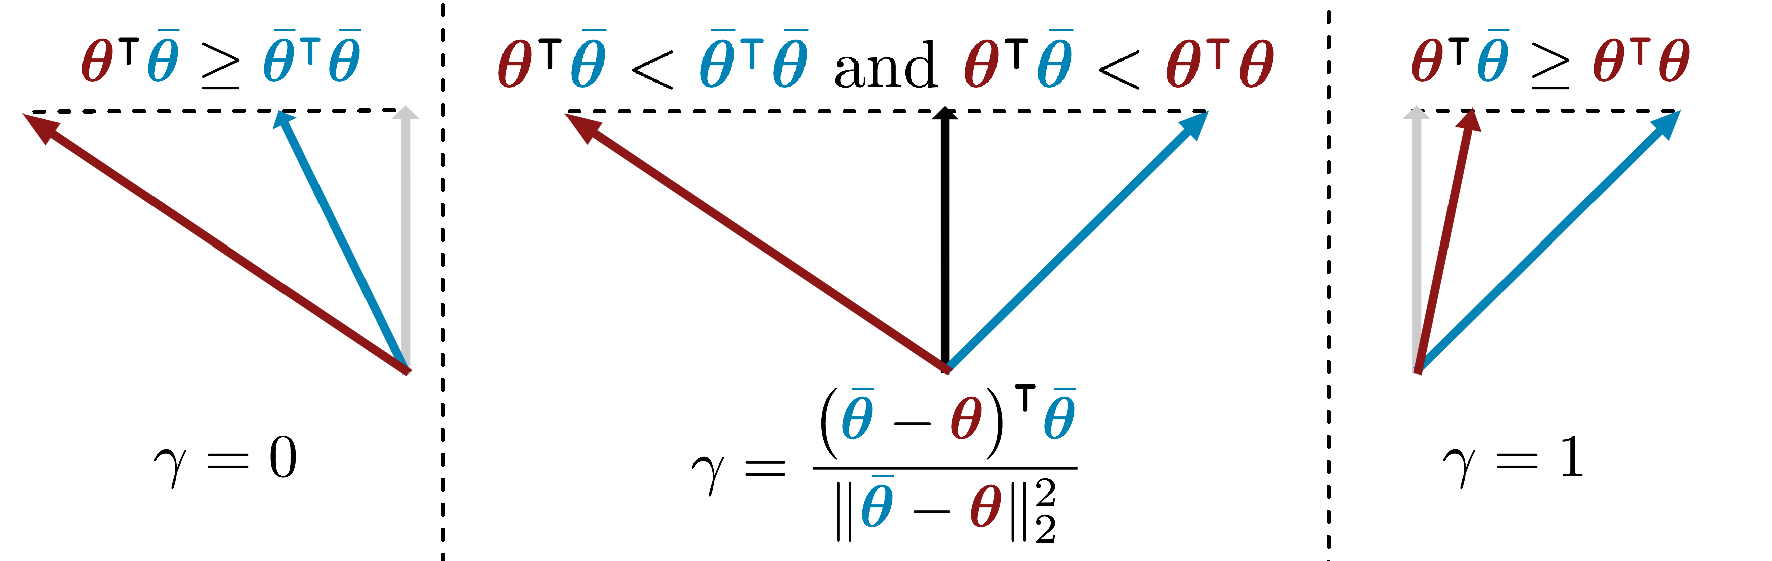
\includegraphics[width=\textwidth]{images/min_norm2point.pdf}
\captionof{figure}{在两点的凸包内寻找最小范数点(\mbox{$\min_{\gamma \in [0,1]} \| \gamma \bm\theta + (1-\gamma) \bar{\bm\theta} \|_2^2$})的可视化。如图所示,解要么出现在边缘,要么解向量垂直于$\bm\theta - \bar{\bm\theta}$。}
\label{fig:min_norm2point}
\end{minipage}
&\begin{minipage}{0.30\textwidth}
\linespread{1.1}
\vspace{-5mm}
\begin{algorithm}[H]\captionsetup{labelsep=newline}
\caption{ $\min_{\gamma \in [0,1]} \| \gamma \bm\theta + (1-\gamma) \bar{\bm\theta} \|_2^2$}
\label{alg:TWO_PNT}
\begin{algorithmic}[1]
\If{$\bm\theta^\intercal \bar{\bm\theta} \geq \bm\theta^\intercal \bm\theta$}
\State $\gamma = 1$
\ElsIf{$\bm\theta^\intercal \bar{\bm\theta} \geq \bar{\bm\theta}^\intercal \bar{\bm\theta}$}
\State $\gamma = 0$
\Else
\State $\gamma = \frac{(\bar{\bm\theta}- \bm\theta)^\intercal \bar{\bm\theta}}{\|\bm\theta - \bar{\bm\theta}\|_2^2}$
\EndIf
\end{algorithmic}
\end{algorithm}
\end{minipage}
\end{tabular}

\begin{algorithm}[H]
\caption{MTL更新算法}
\label{alg:mtl_mgda}
\begin{algorithmic}[1]
\For{$t=1$ {\bfseries to} $T$}
\State $\bm\theta^t = \bm\theta^t - \eta \nabla_{\bm\theta^{t}}  \hat{\mathcal{L}}^t(\bm\theta^\mathrm{sh},\bm\theta^t)$  \Comment{在任务专属权值上进行梯度下降}
\EndFor
\State $\alpha^1,\ldots,\alpha^{T}$ = \textproc{FrankWolfeSolver}($\bm\theta$) \Comment{求解式(\ref{eq:kkt_opt}),得到一个共同的下降方向}
\State $\bm\theta^\mathrm{sh} = \bm\theta^\mathrm{sh} -   \eta \sum_{t=1}^T \alpha^t \nabla_{\bm\theta^\mathrm{sh}}  \hat{\mathcal{L}}^t(\bm\theta^\mathrm{sh},\bm\theta^t)$ \Comment{在任务共享权值上进行梯度下降}
\Statex
\Procedure{FrankWolfeSolver}{$\bm\theta$}
\State Initialize $\bm{\alpha} = (\alpha^1, \ldots, \alpha^{T}) = (\frac{1}{T}, \ldots, \frac{1}{T})$
\State Precompute $\mathbf{M}$ st. $\mathbf{M}_{i,j} = \big(\nabla_{\bm\theta^\mathrm{sh}}  \hat{\mathcal{L}}^i(\bm\theta^\mathrm{sh},\bm\theta^i)\big)^\intercal \big(\nabla_{\bm\theta^\mathrm{sh}}  \hat{\mathcal{L}}^j(\bm\theta^\mathrm{sh},\bm\theta^j)\big)$
\Repeat
\State $\hat{t} = \mathrm{argmin}_r \sum_t \alpha^t \mathbf{M}_{rt}$
\State $\hat{\gamma} = \mathrm{argmin}_{\gamma}  \big( (1 - \gamma) \bm{\alpha} + \gamma \bm{e}_{\hat{t}}  \big)^\intercal \mathbf{M}  \big( (1 - \gamma) \bm{\alpha} + \gamma \bm{e}_{\hat{t}}  \big)$ \Comment{使用算法~\ref{alg:TWO_PNT}求解}
\State $\bm{\alpha} = (1- \hat{\gamma})\bm{\alpha} + \hat{\gamma} \bm{e}_{\hat{t}}$
\Until{$\hat{\gamma} \sim 0$ {\bfseries or} Number of Iterations Limit}
\State {\bfseries return} $\alpha^1,\ldots,\alpha^{T}$
\EndProcedure
\end{algorithmic}
\end{algorithm}

到这里,其实已经有一个非常可用的MTL算法了。但是\citet{Sener18Pareto}还是不太满意,他们对一个encoder-decoder模型提出了一个有效率的算法。算法~\ref{alg:mtl_mgda}需要计算每个任务$t$的$\nabla_{\bm\theta^\mathrm{sh}}  \hat{\mathcal{L}}^t(\bm\theta^\mathrm{sh},\bm\theta^t)$,这样需要在共享权值上对每个任务进行一次反向传播流程。因此,所得梯度的计算过程就是一次前向传播流程和随之而来的$T$次反向传播流程。考虑到反向传播的代价一般比前向传播高,算法~\ref{alg:mtl_mgda}的时间复杂度是$O(T)$。

\citet{Sener18Pareto}又提出了一个优化了式~\ref{eq:kkt_opt}的目标的上界的算法,并且只需要一次反向传播。算法将一个共享表示函数和任务专属的决策函数结合为复合函数,作为假设类的建模和约束:
\begin{equation}
    f^t(\mathbf{x};\bm\theta^\mathrm{sh},\bm\theta^t) = (f^t(\cdot; \bm\theta^t) \circ g(\cdot; \bm\theta^\mathrm{sh})) (\mathbf{x})  = f^t( g(\mathbf{x}; \bm\theta^\mathrm{sh}); \bm\theta^t),
\end{equation}
其中$g$共享表示函数,$f^t$是将共享表示作为输入的任务专属函数。如果我们将共享表示写成$\mathbf{Z} = \left(\mathbf{z}_1,\ldots , \mathbf{z}_N\right)$,其中$\mathbf{z}_i = g(\mathbf{z}_i;\bm\theta^\mathrm{sh})$,那么我们可以定义目标的上界为链式法则的结果:
\begin{equation}
    \Bigg\| \sum_{t=1}^T \alpha^t \nabla_{\bm\theta^\mathrm{sh}}  \hat{\mathcal{L}}^t(\bm\theta^\mathrm{sh},\bm\theta^t) \Bigg\|_2^2  \leq    \Bigg\|\frac{\partial \mathbf{Z}}{\partial \bm\theta^\mathrm{sh}}\Bigg\|_2^2 \Bigg\| \sum_{t=1}^T \alpha^t  \nabla_{\mathbf{Z}}  \hat{\mathcal{L}}^t(\bm\theta^\mathrm{sh},\bm\theta^t) \Bigg\|_2^2,
\end{equation}
其中,$\left\|\frac{\partial \mathbf{Z}}{\partial \bm\theta^\mathrm{sh}}\right\|_2$是$\mathbf{Z}$关于$\bm\theta^\mathrm{sh}$的Jacobian矩阵的范数。对于这个上界有两个良好性质:(1) 可以在一次反向传播中计算所有任务的$\nabla_{\mathbf{Z}} \hat{\mathcal{L}}^t(\bm\theta^\mathrm{sh},\bm\theta^t)$,(2) $\left\|\frac{\partial \mathbf{Z}}{\partial \bm\theta^\mathrm{sh}}\right\|_2^2 $不是关于$\alpha^1,\ldots ,\alpha^T$的函数,因此这一项作为优化的目标可以被移除,得:
\begin{equation}
\min_{\alpha^1,\ldots,\alpha^T}  \Bigg\{  \bigg\| \sum_{t=1}^T \alpha^t  \nabla_{\mathbf{Z}}  \hat{\mathcal{L}}^t(\bm\theta^\mathrm{sh},\bm\theta^t) \bigg\|_2^2 \bigg |  \sum_{t=1}^T \alpha^t = 1, \alpha^t \geq 0 \quad \forall t \Bigg\}
\label{eq:approx}
\end{equation}

这个问题被称为MGDA-UB(Multiple Gradient Descent Algorithm -- Upper Bound),总之他将每个任务关于共享权值$\bm\theta^\mathrm{sh}$的梯度改换成了关于共享表示$\mathbf{Z}$的梯度,并运用改进后的算法~\ref{alg:mtl_mgda}对参数进行更新。然后作者证明,这个问题的解也满足\citet{Desideri12MGDA}的结论,即要么该优化问题的解为$0$且结果点是帕累托静态点并满足KKT条件,要么该解给出了改进所有任务的梯度下降方向。只要$\frac{\partial\mathbf{Z}}{\partial\bm\theta^\mathrm{sh}}$是满秩的,那么这个上界便成立。

\subsection{实现}

\subsubsection{\citefullauthor{Kendall18Uncertainty}}

官方实现是一个空的仓库,很有意思……(GitHub: \href{https://github.com/dyz-zju/multitaskvision}{dyz-zju/multitaskvision},该地址疑为fork过后的)有非官方实现(GitHub: \href{https://github.com/ranandalon/mtl}{ranandalon/mtl}, \href{https://github.com/Mikoto10032/AutomaticWeightedLoss}{Mikoto\-10032/Automatic\-Weighted\-Loss})。

下面是来自Mikoto\-10032/Automatic\-Weighted\-Loss仓库的核心代码和使用示范:
\begin{minted}[
    frame=lines,
    linenos
]{python}
import torch
import torch.nn as nn

class AutomaticWeightedLoss(nn.Module):
    """automatically weighted multi-task loss
    Params:
        num: int,the number of loss
        x: multi-task loss
    Examples:
        loss1=1
        loss2=2
        awl = AutomaticWeightedLoss(2)
        loss_sum = awl(loss1, loss2)
    """
    def __init__(self, num=2):
        super(AutomaticWeightedLoss, self).__init__()
        params = torch.ones(num, requires_grad=True)
        self.params = torch.nn.Parameter(params)

    def forward(self, *x):
        loss_sum = 0
        for i, loss in enumerate(x):
            loss_sum += 0.5 / (self.params[i] ** 2) * loss + \
                torch.log(1 + self.params[i] ** 2)
        return loss_sum

# Demo
from torch import optim

model = Model()
optimizer = optim.Adam([
                {'params': model.parameters()},
                {'params': awl.parameters(), 'weight_decay': 0} # important!
            ])

for i in range(epoch):
for data, label1, label2 in data_loader:
    # forward
    pred1, pred2 = Model(data)
    # calculate losses
    loss1 = loss_1(pred1, label1)
    loss2 = loss_2(pred2, label2)
    # weigh losses
    loss_sum = awl(loss1, loss2)
    # backward
    optimizer.zero_grad()
    loss_sum.backward()
    optimizer.step()
\end{minted}

\subsubsection{\citefullauthor{Chen18GradNorm}}

没有找到官方实现。有一些非官方实现(GitHub: \href{https://github.com/hosseinshn/GradNorm}{hosseinshn/GradNorm}、\href{https://github.com/brianlan/pytorch-grad-norm}{brianlan/pytorch-grad-norm}(简易版)、\href{https://github.com/brianlan/complex-grad-norm}{brianlan/complex-grad-norm}(复杂版))。

下面是本人仿写的代码:
\begin{minted}[
    frame=lines,
    linenos
]{python}
import torch
import torch.nn as nn
import torch.optim as optim

class GradNormLoss(nn.Module):
    def __init__(self, num_of_task, alpha=1.5):
        super(GradNormLoss, self).__init__()
        self.num_of_task = num_of_task
        self.alpha = alpha
        self.w = nn.Parameter(torch.ones(num_of_task, dtype=torch.float))
        self.l1_loss = nn.L1Loss()
        self.L_0 = None

    # standard forward pass
    def forward(self, L_t: torch.Tensor):
        # initialize the initial loss `Li_0`
        if self.L_0 is None:
            self.L_0 = L_t.detach() # detach
        # compute the weighted loss w_i(t) * L_i(t)
        self.L_t = L_t
        self.wL_t = L_t * self.w
        # the reduced weighted loss
        self.total_loss = self.wL_t.sum()
        return self.total_loss

    # additional forward & backward pass
    def additional_forward_and_backward(self, grad_norm_weights: nn.Module, 
            optimizer: optim.Optimizer):
        # do `optimizer.zero_grad()` outside
        self.total_loss.backward(retain_graph=True)
        # in standard backward pass, `w` does not require grad
        self.w.grad.data = self.w.grad.data * 0.0

        self.GW_t = []
        for i in range(self.num_of_task):
            # get the gradient of this task loss with respect to the shared parameters
            GiW_t = torch.autograd.grad(
                self.L_t[i], grad_norm_weights.parameters(),
                    retain_graph=True, create_graph=True)
            # compute the norm
            self.GW_t.append(torch.norm(GiW_t[0] * self.w[i]))
        self.GW_t = torch.stack(self.GW_t) # do not detatch
        self.bar_GW_t = self.GW_t.detach().mean()
        self.tilde_L_t = (self.L_t / self.L_0).detach()
        self.r_t = self.tilde_L_t / self.tilde_L_t.mean()
        grad_loss = self.l1_loss(self.GW_t, self.bar_GW_t * (self.r_t ** self.alpha))
        self.w.grad = torch.autograd.grad(grad_loss, self.w)[0]
        optimizer.step()

        self.GW_ti, self.bar_GW_t, self.tilde_L_t, 
            self.r_t, self.L_t, self.wL_t = None, None, None, None, None, None
        # re-norm
        self.w.data = self.w.data / self.w.data.sum() * self.num_of_task

# This is AN interface.
class GradNormModel:
    def get_grad_norm_weights(self) -> nn.Module:
        raise NotImplementedError(
            "Please implement the method `get_grad_norm_weights`")
\end{minted}

\subsubsection{\citefullauthor{Sener18Pareto}}

有官方实现(GitHub: \href{https://github.com/intel-isl/MultiObjectiveOptimization}{intel-isl/MultiObjectiveOptimization})。

\section{结果与观感}

\subsection{\citefullauthor{Kendall18Uncertainty}}

有很多证据表明这个方法并不那么有效,不过至少提供了个思路。

对于我的任务而言,效果不是很好,只在一个loss取得了不错的效果,其它几个loss有明显的退步。

\subsection{\citefullauthor{Chen18GradNorm}}

没有官方实现导致其价值大大降低。不过根据第三方实现,可以参考实现出一份符合原论文的代码。

对于我的任务而言,效果尚可。只在一个loss取得了不错的效果,其它几个loss有一些退步。

\subsection{\citefullauthor{Sener18Pareto}}

\bibliography{ref/note_20210609}

\end{document}